\documentclass[10pt,a4paper,conference]{IEEEtran}

\usepackage{color}
\usepackage{amsmath}
\usepackage{algorithm}
\usepackage{algorithmic}
\usepackage{threeparttable}
\usepackage[normalem]{ulem}
\usepackage[colorinlistoftodos]{todonotes}

\ifCLASSINFOpdf
\else
\fi

\hyphenation{}


\begin{document}

\title{Estimating Prediction Qualities without 
Ground Truth: A Revisit of the Reverse Testing Framework}

\author{\IEEEauthorblockN{Dheeraj Bhaskaruni}
\IEEEauthorblockA{Department of Computer Science\\
University of Wyoming\\
Laramie, Wyoming, USA\\
Email: vbhaskar@uwyo.edu}
\and
\IEEEauthorblockN{Fiona Patricia Moss}
\IEEEauthorblockA{Department of Computer Science\\
University of Wyoming\\
Laramie, Wyoming, USA\\
Email: fmoss1@uwyo.edu} 
\and 
\IEEEauthorblockN{Chao Lan}
\IEEEauthorblockA{Department of Computer Science\\
University of Wyoming \\ 
Laramie, Wyoming, USA\\
Email: clan@uwyo.edu} 
}

\maketitle

\begin{abstract}
To evaluate prediction qualities of machine learning models, 
it is typically assumed testing samples are labeled. 
However, testing labels are not always available in practice. 
A traditional solution is to approximate prediction qualities 
on testing samples by the qualities on labeled training samples. 
But this may be limited in that it completely ignores 
testing samples. 

In this paper, we present a new approach to estimate prediction 
qualities on unlabeled testing sample, based on the reverse 
testing framework \cite{fan2006reverse}. 
We evaluate the approach with various quality metrics in classification 
and anomaly detection tasks, and over numerous real-world data sets. 
Experimental results show the proposed approach gives a more 
accurate estimate of prediction qualities on testing sample than 
those on training samples. 
\end{abstract}


\IEEEpeerreviewmaketitle

\section{Introduction}

Model assessment is a fundamental task in machine learning. 
To evaluate prediction qualities of models on a testing sample, it is typically assumed the sample is labeled. 
However, this assumption is not always true in practice, 
especially as new testing instances are continuously collected 
faster than one can manually label them. How to estimate 
prediction qualities on unlabeled testing sample? This is 
a research question with significant value in practice. 

A common approach is to approximate testing qualities\footnote{To 
facilitate discussion, we will call 
prediction qualities on testing sample \textit{testing qualities}, 
and those on training sample \textit{training qualities}.} 
by training qualities, presuming a stationary setting. 
However, this may be limited in that it completely ignores 
testing samples. 

A more promising approach is to develop testing-dependent
estimates of testing qualities. However our inspection shows 
its literature appears very sparse, and none of them directly 
addresses the above question. 
Fan and Davidson \cite{fan2006reverse} propose a reverse testing 
framework for model selection; it approximates the comparative 
qualities of two models on testing sample by their reversed 
comparative qualities on training sample. However, the study does 
not address how to assess a single model on unlabeled testing sample. 
Valindria et al. \cite{valindria2017reverse} propose 
a similar approach which approximates a model's segmentation quality 
on a single image by the its reversed segmentation quality on labeled 
training image. However, their problem setting is different from 
the statistical setting addressed in this paper. 
Finally, all above works only examine classification error, while 
there are many other model assessment metrics such as f1-score, 
predictive disparity \cite{hardt2016equality} and AUC score. 
Therefore, how to estimate prediction qualities on unlabeled 
testing sample remains a fairly open question. 

In this paper, we present a new approach to estimate prediction 
qualities on unlabeled testing sample, based on the reverse testing framework introduced by Fan and Davidson \cite{fan2006reverse}. 
The idea is straightforward: 
given a labeled training set and a unlabeled testing set,
one first learns a model from the training set and applies it
to label the testing set; then, one retrains the model on the 
pseudo-labeled testing set and evaluates its prediction qualities 
on the training set -- we call these qualities \textit{reversed 
testing qualities}. 
We hypothesize the reversed testing qualities are more accurate 
estimates of the testing qualities than traditional training qualities.

To verify the above hypothesis, we evaluate proposed approach 
with a variety of quality metrics in classification and anomaly 
detection tasks, including classification error, f1-score, 
predictive disparity and AUC score. We experiment on eight real-world 
data sets, and results show the proposed reversed testing qualities 
are more accurate estimate of the actual testing qualities than 
traditional training qualities. 

The rest of this paper is organized as follows: in section
II, we introduce related background; in section III, we present 
the proposed reverse testing estimators; experimental results 
are presented in section IV, and conclusions are in section V.


\section{Background}

Suppose one learns a prediction model $f: X \rightarrow 
Y$ from a training sample $S \subseteq X \times Y$ and wants 
to evaluate it on a testing sample $Q$. 
Assume label set is binary and $Y = \{-, +\}$. 

We will introduce several metrics of prediction quality, 
and briefly revisit the reverse testing framework. 

\subsection{Common Classification Quality Metrics}

The most common metric of classification quality is 
\textbf{classification error}. If testing sample is labeled 
i.e., $Q \subseteq X \times Y$, the classification error of 
$f$ on $Q$ is 
\begin{equation}
\label{er_test}
er(f; Q) = \frac{1}{|Q|} \sum_{(x, y) \in Q} 
{\bf 1}_{f(x) \neq y}.
\end{equation}

Another common metric is \textbf{f1-score}, 
which is particularly useful when $Y$ has imbalanced classes. 
If the testing sample is labeled, the f1-score of $f$ on $Q$ 
(w.r.t. positive class) is 
\begin{equation}
\label{f1_test}
f1(f; Q) = \frac{2 \cdot pre(f; Q) \cdot rec(f; Q)}{
pre(f; Q) + rec(f; Q)},    
\end{equation}
where $pre$ and $rec$ are precisions and recalls 
defined as 
\begin{equation}
\label{precision}
pre(f; Q) = \frac{\sum_{(x,y) \in Q} {\bf 1}_{f(x) = +, y = +}
}{\sum_{(x,y) \in Q} {\bf 1}_{f(x)=+}}
\end{equation}
and 
\begin{equation}
\label{recall}
rec(f; Q) = \frac{\sum_{(x,y) \in Q} {\bf 1}_{f(x) = +, y = +}
}{\sum_{(x,y) \in Q} {\bf 1}_{y=+}}. 
\end{equation}

From (\ref{er_test}, \ref{precision}, \ref{recall}), we see 
one needs testing labels to estimate $er(f; Q)$ and $f1(f; Q)$; 
and when the labels are not available, the traditional approach 
is to approximate them with $er(f; S)$ and $f1(f; S)$, respectively. 

\subsection{Predictive Demographic Disparity in Classification}

An emerging concern in machine learning is demographic disparity 
in model predictions. For example, a study by Larson et al. 
\cite{larson2016} shows the widely-used recidivism prediction 
software COMPAS has significant racial bias i.e., it mis-predicts 
certain defendants who do not recidivate as high risk re-offenders, 
and this rate for black defendant is twice as often as for white defendant (45\% vs. 23\%). 
In another instance, Klare et al. show several commercialized 
facial recognition algorithms have significant gender bias, 
with males recieving 12\% higher true accept rate compared 
to females \cite{klare2012face}. How to detect and reduce 
predictive disparity is a pressing problem.

An important metric to evaluate demographic disparity in prediction 
is introduced by Hardt et al. \cite{hardt2016equality}, which we 
will call \textbf{conditional predictive disparity}. 
Suppose $Q$ is partitioned into two groups $Q_{1}$ and $Q_{2}$. 
In $Q_{i}$, let $Q_{i+}$ be its subset with positive labels and 
$Q_{i-}$ be its subset with negative labels. 
The conditional predictive disparity is characterized by two ratios 
\begin{equation}
\label{gamma1}
\gamma_{+}(f; Q) = \frac{\Pr \{ f(x) = + \mid x \in Q_{1+} 
\}}{\Pr \{ f(x) = + \mid x \in Q_{2+} \}},  
\end{equation}
and 
\begin{equation}
\label{gamma2}
\gamma_{-}(f; Q) = \frac{\Pr \{ f(x) = + \mid x 
\in Q_{1-} \}}{\Pr \{ f(x) = + \mid x \in Q_{2-} \}}.   
\end{equation}

A model's prediction is considered less biased if $\gamma_{+}(f; Q)$ 
and $\gamma_{-}(f; Q)$ are close to 1. 

From (\ref{gamma1}) and (\ref{gamma2}), we see one needs testing 
labels to estimate $\gamma_{\pm}(f; Q)$; and when the labels are 
not given, the traditional approach is to approximate them using 
$\gamma_{\pm}(f; S)$. 

\subsection{Anomaly Detection Quality Metric}

Anomaly detection is an important task with broad applications 
such as fraud transaction detection, network intrusion detection, 
system fault detection, etc \cite{chandola2009anomaly}. 
A typical detection model $f$ predicts anomalous scores of 
testing instances, and thresholds them to identify anomalous 
instances. 

A common metric of detection quality is {\bf AUC score}, 
where the ROC curve is drawn with x-axis being the false alarm 
rate and y-axis being the detection rate. 
Suppose anomalous instances are labeled positive and normal 
ones are labeled negative. Let $f(x;r)$ be a detection 
model with anomalous scores thresholded by $r$, 
such that $f(x; r) = +$ if $f(x) > r$ and $f(x; r) = -$ 
otherwise.  The AUC score of $f$ on $Q$ is 
\begin{equation}
AUC(f; Q) = \sum_{r} dr(f; Q, r) \cdot \Delta far(f; Q, r),  
\end{equation}
where $dr$ and $far$ are detection rate and false alarm rate 
(w.r.t. threshold $r$), respectively, defined as 
\begin{equation}
\label{addr}
dr(f; Q, r) = 
\frac{\sum_{(x,y) \in Q} {\bf 1}_{f(x; r) = +, y = +}}{
\sum_{(x,y) \in Q} {\bf 1}_{y = +}}, 
\end{equation}
and 
\begin{equation}
\label{adfar}
far(f; Q, r) = 
\frac{\sum_{(x,y) \in Q} {\bf 1}_{f(x; r) = +,  
y = -}}{\sum_{(x,y) \in Q} {\bf 1}_{y = -}}. 
\end{equation}

(\ref{addr}) and (\ref{adfar}) suggest one needs testing 
labels to estimate AUC score; and one can approximate them 
using $dr(f; S, r)$ and $far(f; S, r)$ in case testing labels 
are not available. 

\subsection{The Reverse Testing Framework: A Revisit}

The reverse testing framework is proposed for model 
selection in non-stationary setting by Fan and Davidson \cite{fan2006reverse}. 
It assesses comparative prediction qualities of two models 
on testing sample through a reverse testing process: 
it first learns two models from $S$ and applies them to 
label $Q$; then it retrains the two models on the 
pseudo-labeled $Q$ and evaluates them on $S$. Their hypothesis 
is that a model with higher prediction quality on $S$ has 
higher prediction quality on $Q$. 

Fan's approach does not apply to the problem studied 
in this paper. It assesses comparative performance 
between two models, while this paper aims to assess 
performance of a single model. 
In addition, it only examines classification error, 
while this paper additionally examines f1-score, 
predictive disparity and AUC score. 
However, our proposed approach is largely motivated 
by Fan's work. 




\section{Estimating Testing Qualities based on A 
Reverse Testing Framework} 

In this section, we propose approaches to estimate 
testing qualities without testing labels. 
The idea is straightforward: one first learns a model 
from training set, and applies it to label the testing 
set; then one re-trains the model on the pseudo-labeled 
testing set, and evaluates its prediction qualities on 
the training set. We will call the later 
\textit{reversed testing qualities} and hypothesize 
they are good estimate of the testing qualities. 

Our approaches for classification and anomaly detection 
tasks are slightly different, and will be introduced 
separately. 

For classification, let $M$ be a metric of prediction 
quality. It can be classification error $er(f; Q)$, 
f1-score $f1(f; Q)$ or conditional prediction 
disparities $\gamma_{+}(f; Q)$ and $\gamma_{-}(f; Q)$. 
Our proposed estimation approach is described in 
Algorithm \ref{alg:prediction}. Note it does not require 
labels of testing sample. 

\begin{algorithm}[h]
\begin{algorithmic}
   \STATE {\bfseries Input:} Labeled training set $S$, 
   Unlabeled testing set $Q$, Model $f$, 
   Prediction quality metric $M$
   \STATE 1: train $f$ on $S$ and apply it to label $Q$ \\   
   \STATE 2: retrain $f$ on pseudo-labeled $Q$ 
   \STATE 3: evaluate $f$ on $S$ based on metric $M$
   \STATE {\bfseries Output:} prediction quality 
   of $f$ on $S$ (as an estimate of $f$'s prediction 
   quality on $Q$)  
   \vskip -0.2in
\end{algorithmic}
   \caption{Reversed Classification Quality Estimator}
\label{alg:prediction}
\end{algorithm}

For anomaly detection, $M$ is AUC score $AUC(f; Q)$. 
Our proposed estimation approach is described in 
Algorithm \ref{alg:anomalydetection}. 

\begin{algorithm}[h]
\begin{algorithmic}
   \STATE {\bfseries Input:} Labeled training set $S$, 
   Unlabeled testing set $Q$, Model $f$, Detection 
   threshold $r$  
   \STATE 1: train $f$ on {normal instances} in $S$ 
   and apply  it to detect anomalies in $Q$ based on 
   threshold $r$ \\   
   \STATE 2: retrain $f$ on pseudo-labeled normal instances 
   in $Q$ 
   \STATE 3: evaluate $f$ on $S$ and obtained detection 
   rate and false alarm rate based on $r$ 
   \STATE 4: repeat step 1-3 with different threshold 
   $r$ to obtain AUC score of $f$ on $S$ 
   \STATE {\bfseries Output:} AUC score of $f$ on $S$
    (as an estimate of $f$'s AUC score on $Q$)
   \vskip -0.2in
\end{algorithmic}
   \caption{Reversed Anomaly Detection Quality Estimator}
\label{alg:anomalydetection}
\end{algorithm}

Algorithm \ref{alg:anomalydetection} does not require labels of 
testing set. It differs from Algorithm \ref{alg:prediction} 
in that it trains and retrains the model only on normal 
instances and with different threshold values. 

\section{Experiment}

\subsection{Data Description and Experimental Protocol}

In this section, we introduce seven experimented data sets 
and experimental protocols.

Three data sets are security related. One is the Spam Email 
data set downloaded from the UCI data repository; 
it contains 4601 profiled emails categorized into spam emails 
and normal emails. Another one is the Big Malware 
classification Challenge 2015 data set downloaded 
from Kaggle 
\footnote{https://www.kaggle.com/c/malware-classification}; 
it contains approximately 10,000 profiled malware files that 
are categorized into nine families, including Ramnit, 
Lollipop, Vundo, etc. The third one is the Coburg Intrusion Detection data set recently created by Ring et al. 
\cite{ring2017flow}; it contains approximately 
32 million profiled network flows collected in a 
period of 4 weeks and categorized into five classes, 
namely, attack, normal, suspicious, unknown and victim. 

The other four data sets are widely used for anomaly 
detection task, and are downloaded from Stony Brook 
University's Outlier Detection DataSets\footnote{http://odds.cs.stonybrook.edu/}. 
One is the Satellite data set; it contains 6435 
profiled patches of satellite images that are divided 
into 36 different classes, including red soil, cotton crop, 
grey soil,etc. Another one is the Ionosphere data set; 
it contains 351 profiled radar-transmitted signals that 
are classified into anomalous and normal signals. 
The third one is the Cardio data set; it contains 1831 
profiled patients classified into anomalous, suspect and 
normal patients. The last one is Arrhythmia data set; 
it contains 452 profiled patients with or without the 
presence of cardiac arrhythmia. 

To examine predictive demographic disparity, we 
collected the Crime Community data set \cite{redmond2002data}. 
It contains 1994 profiled U.S. communities 
labeled by their recorded violent crime rates. 
We binarized crime rates such that those above 50\% (high-risk 
communities) were encoded as 1, and those below 50\% (low-risk communities) were encoded as -1. 

All categorical features were encoded by dummy variables. 

In each experiment, we randomly chose 50\% instances on 
a data set for training and used the rest for testing. 
We repeated the random trials for 20 times, and reported 
the averaged prediction qualities. Hyper-parameters of 
all models were optimized through grid search, 
and those yielding optimal testing performance were selected. 



\subsection{Estimate Classification Qualities without 
Testing Labels} 

In this section, we evaluate Algorithm \ref{alg:prediction} 
with four representative prediction models, namely, 
logistic regression, linear SVM, k-nearest neighbor 
and decision tree. 

We will first present a case study on the Spam Email data 
set, and then present extensive results on other data sets. 

{\noindent \bf A Case Study on Spam Email Data Set} 

We examined logistic regression on the Spam Email 
data set. The regularization coefficient of logistic 
regression was set to 10 based on 
our grid search results in Figure \ref{exp1:modelselection}. 

\begin{figure}[h]
\centering
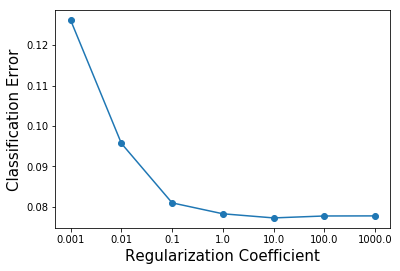
\includegraphics[width=4.5cm,height=3.25cm]{exp1_modelselection.png}
\vspace{-10pt}
\caption{Testing Error versus Regularization Coefficient}
\label{exp1:modelselection}
\end{figure}

First, we evaluated classification error. 
Recall $er(f; Q)$ is the testing error. 
Let $er(f; S)$ be the training error, and 
$\tilde{er}(f; S)$ be the reversed testing error. 
The estimation quality of $er(f; S)$ on $er(f; Q)$ 
is measured by 
\begin{equation}
\Delta_{tr} = | er(f; Q) - er(f; S)  |,  
\end{equation}
and the estimation equality of $\tilde{er}(f; S)$ 
on $er(f; Q)$ is 
\begin{equation}
\Delta_{retr} = | er(f; Q) - \tilde{er}(f; S) |.  
\end{equation}
Results are shown in Table \ref{exp1:classificationerror}. 
We see $\tilde{er}(f; S)$ is closer to $er(f; Q)$ 
than $er(f; S)$, which is a first empirical evidence 
that reversed testing quality is a more accurate estimate 
of testing quality than traditional training 
quality\footnote{More 
results of this experiment can be found in 
Table \ref{tab1:accf1}.}. 

\begin{table}[h]
\renewcommand{\arraystretch}{1.5} 
\caption{Classification Errors on Spam Email Data Set}
\centering
\begin{tabular}{l|ccccc} \hline 
\bf Metric & \bf $er(f; Q)$ & \bf $er(f; S)$ & \bf 
$\tilde{er}(f; S)$ & \bf $\Delta_{tr}$ & \bf 
$\Delta_{retr}$ \\ \hline 
\bf Value & .0686 & .0773 & .0733 & .0087 & .0040 \\ \hline 
\end{tabular}
\label{exp1:classificationerror}
\end{table}

Next, we evaluated the impact of sample size on 
estimation. We varied the fraction of training 
instances from 10\% to 90\% (with the remaining 
instances used for testing), and obtained results 
in Figure \ref{exp1:samplesize}. 
Wee see $\tilde{er}(f; S)$ remains a more accurate 
estimate of $er(f; Q)$ in most cases, except when 
testing sample is very small (less than 20\% of the 
data set). The latter suggests reversed testing 
quality is more effective when one has sufficient 
testing sample. 

\begin{figure}[h]
\centering
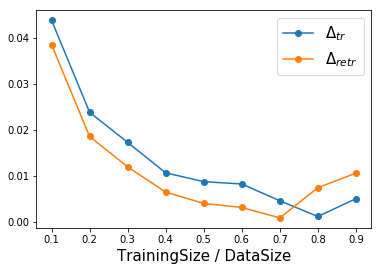
\includegraphics[width=5cm,height=3.5cm]{exp1_samplesize.png}
\vspace{-10pt}
\caption{Performance over Different Training Sample Size}
\label{exp1:samplesize}
\end{figure}

So far, we have been retraining $f$ using all pseudo-labeled 
instances in $Q$. Since some pseudo-labels may be incorrect, 
it is natural to ask whether one can improve reversed 
testing qualities by using only confidently pseudo-labeled 
instances to retrain $f$. Our results in 
Figure \ref{exp1:confidence} suggest this is possible, 
but the improvement seems marginal. 
This may be because unconfidently labeled instances often 
lie around decision boundary, and any learner with proper 
error tolerance would be robust to them during training 
(or retraining). 
The results also suggest one has to maintain a sufficient 
testing sample, because reversed testing quality starts 
to degrade when less than $50\%$ confidently pseudo-labeled
instances are used to retrain $f$. 

\begin{figure}[h]
\centering
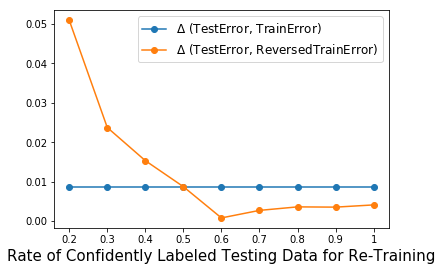
\includegraphics[width=5.5cm,height=3.5cm]{exp1_confidence.png}
\vspace{-10pt}
\caption{$\Delta_{tr}$ and $\Delta_{retr}$ versus Re-training Sample Size}
\label{exp1:confidence}
\end{figure}

{\noindent \bf Results on other data sets based on 
other models} 

Now we evaluate Algorithm \ref{alg:prediction} 
extensively on multiple data sets, based on different 
base models and prediction quality metrics. 
Let $\tilde{f1}(f; S)$ be the reversed f1-score. 
Results are shown in Table \ref{tab1:accf1}. 

We see $\tilde{er}(f; S)$ is a more 
accurate estimate of $er(f; Q)$ than $er(f; S)$, 
and $\tilde{f1}(f; S)$ is a more accurate 
estimate of $f1(f; Q)$ than $f1(f; S)$. 
These observations are consistent across different 
base models and different data sets. 
An exception is on the Malware data set. 
This may be because the testing error on this data set 
is very large (around 0.38), thus pseudo-labels are 
mostly wrong and significantly mislead $f$ in its retraining. 
This suggests reversed testing quality is more effective 
when prediction quality is relatively high. 

































\subsection{Estimate Anomaly Detection Quality 
without Test Label}

In this section, we evaluate Algorithm 
\ref{alg:anomalydetection} 
with four representative anomaly detection models, 
including one-class SVM, PCA, k-means and GMM. 
Again, we first present a case study and then other results. 

\begin{table*}[t]
\centering
\renewcommand{\arraystretch}{1.5}
\caption{Conditional Predictive Demographic Disparity on the 
Crime Community Data Set}
% \centering
\begin{tabular}{l|ccccc|ccccc} \hline 
\bf Classifier & \bf $\gamma_{+}(f; Q)$ & \bf $\gamma_{+}(f; S)$ 
& \bf $\gamma_{+}(f_{q}; S)$ & \bf $\Delta_{tr}$ & 
\bf $\Delta_{retr}$ & \bf $\gamma_{-}(f; Q)$ & \bf $\gamma_{-}(f; S)$ 
& \bf $\gamma_{-}(f_{q}; S)$ & \bf $\Delta_{tr}$ & 
\bf $\Delta_{retr}$ \\ \hline 
LogitRegressor & .316 (4e-3) & .368 (3e-3) & .246 (3e-3) & .052 & .070 
& .034 (2e-4) & .030 (1e-4) & .027 (7e-5) & .004 & .008 \\ 
LSVM & .300 (3e-3) & .376 (4e-3) & .297 (4e-3) & .076 & .003 
& .039 (2e-4) & .024 (2e-4) & .024 (1e-4) & .015 & .014\\ 
k-NN & .290 (4e-3) & .419 (6e-3) & .262 (6e-3) & .129 & .029 
& .056 (4e-4) & .044 (3e-4) & .026 (3e-4) & .012 & .030\\  
DecisionTree & .364 (2e-2) & .451 (2e-3) & .384 (2e-2) & .087 & .020 
& .072 (1e-3) & .060 (2e-3) & .067 (3e-3) & .012 & .004\\  \hline 
\end{tabular}
\label{exp1:disparity}
\end{table*}

{\noindent \bf A Case Study on Spam Email Data Set} 

We formalized an anomaly detection task by considering 
spam emails as anomalies. Recall that only normal 
instances were used to train model at first, but all 
training instances were used to evaluate the retrained model.
One-class linear SVM was used as the base detection model. 
Its regularization coefficient was set to 1e-3 based on 
results in Figure \ref{exp1:anomalymodelselection}. 

\begin{figure}[h]
\centering
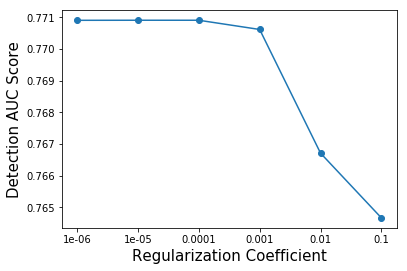
\includegraphics[width=4.5cm,height=3.25cm]{exp1_anomalymodelselection.png}
\vspace{-10pt}
\caption{Testing Error versus Regularization Coefficient}
\label{exp1:anomalymodelselection}
\end{figure}

We evaluated AUC score. Recall $AUC(f; Q)$ is the 
testing score and $AUC(f; S)$ is the training score. 
Let $\widetilde{AUC}(f; S)$ be the reversed testing score. 
The estimation quality of $AUC(f; S)$ on $AUC(f; Q)$ is 
\begin{equation}
\Delta_{tr} = | AUC(f; Q) - AUC(f; S) |,  
\end{equation}
and the estimation equality of $\widetilde{AUC}(f; S)$ 
on $AUC(f; S)$ is 
\begin{equation}
\Delta_{retr} = | AUC(f; Q) - \widetilde{AUC}(f; S) |.  
\end{equation}

Results in Table \ref{exp1:anomalyaucscore} show 
reversed AUC score is a more accurate 
estimate of testing AUC score than training AUC. 

\begin{table}[h]
\renewcommand{\arraystretch}{1.5} 
\caption{Anomaly Detection AUC Scores on Spam Email Data Set}
\centering
\begin{tabular}{ccccc} \hline 
$AUC(f; Q)$ & $AUC(f; S)$ & $AUC(f_{q}; S)$ 
& $\Delta_{tr}$ & $\Delta_{retr}$ \\ \hline 
.7709 & .7733 & .7705 & .0024 & .0004 \\ \hline 
\end{tabular}
\label{exp1:anomalyaucscore}
\end{table}

Next, we evaluated the impact of sample size on 
estimation quality and obtained results in 
Figure \ref{exp1:anomalysamplesize}. 
We see reversed AUC score is more effective when 
training sample and testing sample are more balanced. 
This is different from our observations in 
classification tasks. 

\begin{figure}[h]
\centering
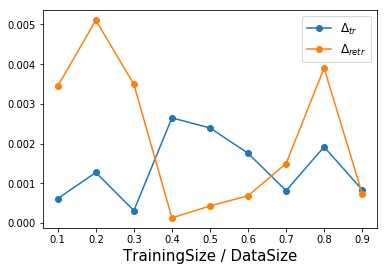
\includegraphics[width=5.5cm,height=3.5cm]{exp1_anomalysamplesize.png}
\vspace{-10pt}
\caption{$\Delta_{tr}$ and $\Delta_{retr}$ versus Training 
Sample Size} 
\label{exp1:anomalysamplesize}
\end{figure}

Finally, we evaluated the impact of label confidence 
on estimation quality. We used $70\%$ data for training 
and the rest for testing. 
We used only confidently pseudo-labeled normal instances 
to retrain $f$, 
and obtained results in Figure \ref{exp1:anomalyconfidence}. 
We see reversed AUC score becomes a better estimate 
as one uses fewer confidently pseudo-labeled instances 
for retraining, but it remains less accurate than 
training AUC score.  

\begin{figure}[h]
\centering
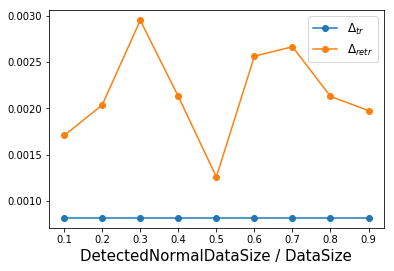
\includegraphics[width=5.5cm,height=3.5cm]{exp1_anomalyconfidence.png}
\vspace{-10pt} 
\caption{$\Delta_{tr}$ and $\Delta_{retr}$ versus Different 
Fractions of Identified Normal Instances. (TraininSize/DataSize=0.7)}
\label{exp1:anomalyconfidence}
\end{figure}

{\noindent \bf Results on other Data Sets with 
other Models} 

Now we evaluate Algorithm \ref{alg:anomalydetection} 
extensively on several data sets based on 
multiple detection models. 
Results are shown in Table \ref{tab1:auc}. 
We see $\widetilde{AUC}(f; S)$ is consistently 
a more accurate estimate of $AUC(f; Q)$ than 
$AUC(f; S)$. 

% \begin{table*}[t!]
% \renewcommand{\arraystretch}{1.5} 
% \caption{Z-Scores of all the data sets used in the experiments}
% \centering
% \begin{tabular}{|l|c|c|c|c|c|c|c|c|} \hline 
% \bf Data Set & Spam Email & Satellite & Cardio & Ionosphere & Malware & Network Intrusion & Arrhythmia \\ \hline 
% \bf Z-Score & 2e-4 & 2e-3 & 5e-4 & 1e-2 & 2e-5 & 4e-5 & 3e-4 \\  \hline 
% \end{tabular}
% \label{exp1:disparity}
% \end{table*}


\subsection{Estimate Conditional Predictive Demographic Disparity without Testing Labels} 

In this section, we evaluate Algorithm \ref{alg:prediction} 
for the conditional predictive disparity on the Crime 
Community data set. 

We examined the disparity between African American (AA) 
and non-African American  (nAA) communities. The former 
are those with feature ``percentage of population that 
is African American'' above 50\%, and the latter 
are the rest communities. 

Recall $\gamma_{\pm}$ are the ratios 
that characterize conditional predictive demographic 
disparity. Let $\tilde{\gamma}_{\pm}$ be the reversed 
testing ratios. The estimation quality of 
$\gamma_{\pm}(f; S)$ on $\gamma_{\pm}(f; Q)$ is 
\begin{equation}
\Delta_{tr} = | \gamma_{\pm}(f; Q) - \gamma_{\pm}(f; S)|, 
\end{equation}
and the quality of $\tilde{\gamma}_{\pm}(f; S)$ 
on $\gamma_{\pm}(f; Q)$ is 
\begin{equation}
\Delta_{retr} = | \gamma_{\pm}(f; Q) 
- \tilde{\gamma}_{\pm}(f; S)|.  
\end{equation}
Results are shown in Table \ref{exp1:disparity}.  
We see $\tilde{\gamma}_{\pm}(f; S)$ are 
more accurate estimate of $\gamma_{\pm}(f; Q)$ 
than $\gamma_{\pm}(f; S)$ in most cases, with 
an exception with logistic regression. 







\subsection{Stationary Assumption} 

The proposed approaches are based on the 
stationary assumption. We verified this 
assumption by computing the z-scores between 
training and testing samples. Results averaged 
over 20 random trails on different data sets 
are 2e-4 for Spam Email, 2e-3 for Satellite, 
5e-4 for Cardio, 1e-2 for Ionosphere, 2e-5 for Malware, 
4e-5 for CID and 3e-4 for Arrhythmia. These results 
suggest there is no significant difference between 
training and testing distributions. 

This paper focuses on stationary setting. 
How to develop estimation approach 
for non-stationary setting is a future direction. 
Fan's work does not seem directly applicable, 
and one may consider combining it with techniques 
for correcting sample selection bias e.g. 
\cite{huang2007correcting}.


% \begin{table*}[t!]
% \renewcommand{\arraystretch}{1.5} 
% \caption{Z-Scores of all the data sets used in the experiments}
% \centering
% \begin{tabular}{|l|c|c|c|c|c|c|c|c|} \hline 
% \bf Data Set & Spam Email & Satellite & Cardio & Ionosphere & Malware & Network Intrusion & Arrhythmia \\ \hline 
% \bf Z-Score & 2e-4 & 2e-3 & 5e-4 & 1e-2 & 2e-5 & 4e-5 & 3e-4 \\  \hline 
% \end{tabular}
% \label{exp1:disparity}
% \end{table*}

\begin{table*}[t!]
\renewcommand{\arraystretch}{1.3} 
\caption{Classification Error and F1 Score Comparison on Six Data Sets}
\centering
\begin{threeparttable}
\setlength{\tabcolsep}{0.35em}
\begin{tabular}{llccccc|ccccc} %
\bf Data Set & \bf Classifier 
& $er(f; Q)$ & $er(f; S)$ & $er(f_{q}; S)$ &  $\Delta_{tr}$ & $\Delta_{retr}$ 
& $f1(f; Q)$ & $f1(f; S)$ & $f1(f_{q}; S)$ &  $\Delta_{tr}$ & $\Delta_{retr}$ \\ \hline 
S-Email & LogReg & .077 (3e-5) & .069 (2e-5) & .073 (2e-5) & .009 & .004  
& .901 (5e-5) & .911 (4e-5) & .905 (3e-5) & .010 & .004  \\ 
\ & LSVM & .189 (4e-5) & .054 (1e-5) & .187 (4e-5) & .135 & .003  
& .766 (5e-5)  & .928 (2e-5) & .774 (8e-5) & .162 & .008   \\ 
\ & kNN & .211 (4e-5) & .110 (3e-5) & .175 (5e-5) & .101 & .036 
& .729 (3e-5) & .858 (8e-5) & .771 (1e-4) & .128 & .042  \\ 
\ & DTree & .096 (4e-5) & .000 (0) & .091 (1e-4) & .096 & .005  
& .880 (6e-5) & .999 (0) & .091 (1e-4) & .120 & .006   \\ \hline 
Satellite & LogReg & .126 (2e-5) & .124 (2e-5) & .124 (3e-5) & .002 & .002  
& .770 (6e-5) & .775 (6e-5) & .774 (9e-5) & .004 & .003  \\  
\ & LSVM & .122 (2e-5) & .121 (2e-5) & .121 (2e-5) & .001 & .001 
& .772 (6e-5) & .775 (5e-5) & .774 (5e-5) & .002 & .002   \\ 
\ & kNN & .081 (3e-5) & .039 (7e-6) & .077 (2e-5) & .042 & .004   
& .871 (6e-5) & .938 (1e-5) & .877 (5e-5) & .066 & .006   \\ 
\ & DTree & .126 (4e-5) & 0 (0) & .129 (1e-4) & .126 & .003  
& .802 (1e-4) & 1 (0) & .799 (3e-4) & .198 & .003   \\ \hline 
Cardio & LogReg & .0120 (1e-5) & .014 (1e-5) & 0.021 (1e-5) & .005 & .001  
& .898 (4e-4) & .924 (3e-4) & .888 (3e-4) & .026 & .010 \\ 
\ & LSVM & .016  (1e-5) & .009 (1e-5) & .014 (1e-5) & .007 & .002
& .914 (3e-4) & .951 (2e-4) & .923 (4e-4) & .036 & .009  \\ 
\ & kNN & .018 (1e-5) & .011 (4e-6) & .019 (9e-6) & .007 & .001 
& .903 (4e-4) & .943 (9e-5) & .892 (2e-4) & .040 & .011 \\ 
\ & DTree & .019 (2e-5) & .004  (3e-6) & .017 (3e-5) & .015 & .003  
& .899 (5e-4) & .977 (6e-5) & .909 (1e-3) & .078 & .010 \\ \hline 
Iono. & LogReg & .143 (5e-4) & .076 (2e-4) & .139 (4e-4) & .067 & .004  
& .764 (1e-3) & .886 (5e-4) & .764 (1e-3) & .122 & .001 \\ 
\ & LSVM & .140 (4e-4) & .089 (1e-4) & .128 (3e-4) & .050 & .012 
& .776 (1e-3) & .866 (2e-4) & .792 (1e-3) & .091 & .017 \\ 
\ & kNN & .156 (1e-3) & .098 (1e-4) & .176 (1e-3) & .059 & .020 
& .733 (2e-3) & .846 (5e-4) & .692 (4e-3) & .114 & .041 \\ 
\ & DTree & .134 (1e-3) & .001 (8e-6) & .108 (8e-4) & .133 & .026  
& .813 (1e-3) & .998 (1e-5) & .845 (1e-3) & .186 & .032 \\ \hline 
Malware & LogReg & .387 (2e-4) & .387 (1e-4) & .438 (1e-4)& .001 & .051  
& .552 (3e-4) & .552 (1e-4) & .487 (4e-4) & .001 &  .065  \\
% \ & LSVM & .709 (8e-3) & .708 (8e-3) & .725 (1e-2) & .001 & .016 
% & .240 (8e-3) & .241 (8e-3) & .228 (1e-2) & .001 & .011  \\ 
\ & kNN & .214 (2e-5) & .119 (1e-5) & .181 (2e-5) & .095 & .033  
& .784 (2e-5) & .880 (1e-5) & .817(1e-5) & .096 & .033 \\  
\ & DTree & .039 (2e-5) & .022 (1e-5) & .041 (2e-5) & .016 & .002  
& .961 (2e-5) & .977 (1e-5) & .959 (2e-5) & .016 & .002 \\ \hline 
CID 
& LogReg & .426 (7e-3) & .423 (7e-3) & .446 (3e-3)& .003 & .020  
& .546 (9e-3) & .549 (9e-3) & .513 (4e-3) & .002 &  .033  \\
\ & LSVM & .316 (6e-5) & .313 (5e-5) & .314 (6e-5) & .003 & .002  
& .614 (6e-5) & .617 (5e-5) & .615 (6e-5) & .003 & .001 \\
\ & kNN & .023 (5e-6) & .013 (1e-6) & .022 (2e-6) & .010 & .001  
& .976 (5e-6) & .987 (1e-6) & .978 (2e-6) & .010 & .001 \\ 
\ & DTree & .025 (6e-6) & .016 (8e-6) & .027 (3e-5) & .009 & .002  
& .975 (6e-6) & .984 (8e-6) & .973 (3e-5) & .009 & .002 \\ \hline 
\end{tabular}
\end{threeparttable}
\label{tab1:accf1}
\end{table*}



\begin{table*}[t!]
\renewcommand{\arraystretch}{1.3} 
\caption{Anomaly Detection AUC Score Comparison on Six Data Sets}
\centering
\begin{threeparttable}
\begin{tabular}{llccccc} %
\bf Data Set & \bf Classifier & \bf $AUC(f; Q)$
& \bf $AUC(f; S)$ & \bf $\widetilde{AUC}(f; Q)$
&  $\Delta_{tr}$ & $\Delta_{retr}$ \\ \hline 
Spam Email & OC-SVM  & .7647 (7e-5) & .7672 (7e-5) 
& .7642 (7e-5) & .0025 & .0005  \\ 
\ & PCA & .8215 (1e-4) & .8372 (3e-4) & .8248 (4e-4) & .0157 & .0033  \\ 
\ & k-means & .7821 (5e-5) & .8666 (2e-5) & .7408 (5e-5) & .0845 & .0413  \\ 
\ & GMM & .7506 (7e-3) & .8282 (8e-5) & .7302 (4e-3) & .0776 & .0204  \\ \hline 
Satellite & OC-SVM & .3040 (3e-5) & .3028 (4e-5) & .3032 (3e-5) & .0012 & .0008  \\ 
\ & PCA & .8010 (5e-5) & .7984 (6e-5) & .7999 (5e-5) & .0026 & .0010  \\ 
\ & k-means & .8816 (3e-5) & .9807 (2e-6) & .8216 (3e-5) & .0991 & .0600 \\ 
\ & GMM & .8605 (7e-5) & .9544 (4e-5) & .8210 (8e-5) & .0939 & .0395 \\ \hline 
Arrhythmia & OC-SVM & .4625 (1e-3) & .4283 (1e-3) & .4512 (3e-3) & .0342 & .0114  \\ 
\ & PCA & .8371 (6e-4) & .8512 (5e-4) & .8341 (8e-4) & .0141 & .0030 \\ 
\ & k-means & .8250 (9e-4) & .9438 (2e-4) & .8162 (1e-3) & .1187 & .0088 \\ 
\ & GMM & .7975 (8e-4) & .9997 (0) & .7769 (2e-3) & .2022 & .0206 \\ \hline 
Iono. & OC-SVM & .1427 (4e-4) & .1235 (5e-4) & .1334 (5e-4) 
& .0193 & .0094  \\ 
\ & PCA & .9577 (2e-4) & .9782 (9e-5) & .9494 (2e-4) & .0205 & .0083 \\ 
\ & k-means & .9639 (3e-4) & .9962 (1e-5) & .9476 (4e-4) & .0323 & .0162 \\ 
\ & GMM & .9272 (2e-3) & .9999 (0) & .9394 (3e-4) & .0727 & .0123 \\ \hline 
Cardio & OC-SVM& .9853 (5e-5) & .9869 (3e-5) & .9857 (4e-5) & .0015 & .0003  \\ 
\ & PCA & .9499 (4e-5) & .9500 (4e-5) & .9461 (4e-5) & .0001 & .0038  \\ 
\ & k-means & .9408  (6e-5) & .9975 (1e-6) & .9030 (6e-5) & .0567 & .0378  \\ 
\ & GMM & .3227 (3e-3) & .8964 (2e-3) & .4159 (3e-3) & .5736 & .0932 \\ \hline 
CID & OC-SVM & .5013 (4e-5) & .4982 (4e-5) & .4982 (4e-5) & .0031 & .0031  \\ 
\ & PCA & .9990 (1e-6) & 1.0000 (0) & .9982 (2e-6) & .001 & .0008  \\ 
\ & k-means & .9909 (3e-6) & .9934 (3e-6) & .9922 (3e-6) & .0024 & .0013  \\ 
\ & GMM & .9980 (1e-6) & .9977 (1e-6) & .9905 (1e-6) & .0003 & .0072 \\ \hline 
\end{tabular}
\end{threeparttable}
\label{tab1:auc}
\end{table*}


\section{Conclusion}

In this paper, we propose a new approach to estimate 
prediction qualities on unlabeled testing sample. 
We show this approach gives a more accurate estimate of 
testing qualities than traditional training qualities 
in both classification and anomaly detection tasks, 
under four common quality metrics including 
classification error, f1-score, predictive demographic 
disparity and AUC score. 





\bibliographystyle{IEEEtran}
\bibliography{reference}

\end{document}




%\begin{figure}[h]
%\centering
%\includegraphics[width=.25\textwidth]{Backward_data_training.PNG} 
%\caption{Backward data evaluation Training}
%\end{figure}

